\section{Cooperative Class Reference}
\label{class_cooperative}\index{Cooperative@{Cooperative}}
Inheritance diagram for Cooperative::\begin{figure}[H]
\begin{center}
\leavevmode
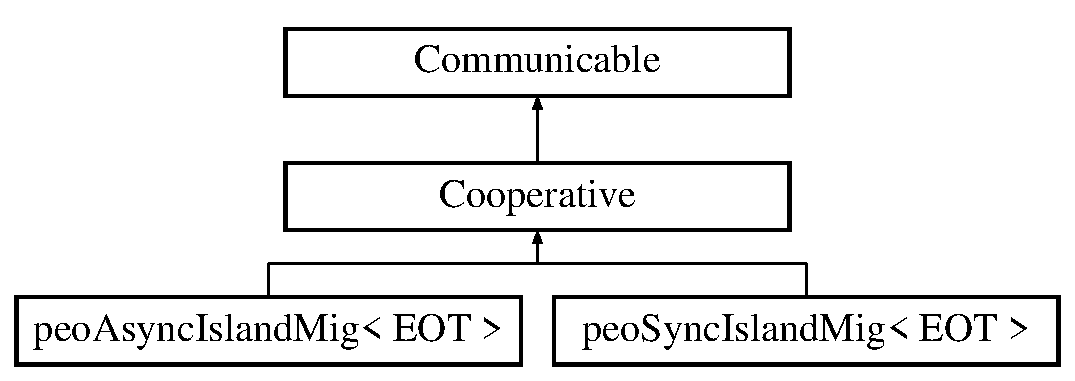
\includegraphics[height=3cm]{class_cooperative}
\end{center}
\end{figure}
\subsection*{Public Member Functions}
\begin{CompactItemize}
\item 
{\bf Runner} $\ast$ {\bf get\-Owner} ()\label{class_cooperative_4012b4e8329e87d26ee266491e1a883e}

\item 
void {\bf set\-Owner} ({\bf Runner} \&\_\-\_\-runner)\label{class_cooperative_fe7b022567174c8305bc78d8c5749b12}

\item 
virtual void {\bf pack} ()=0\label{class_cooperative_6a4848c94031289df281a571ea427d46}

\item 
virtual void {\bf unpack} ()=0\label{class_cooperative_7c31a68fb29e0a9cbe1da8019e4cdafa}

\item 
void {\bf send} ({\bf Cooperative} $\ast$\_\-\_\-coop)\label{class_cooperative_c609f2a1200da7d1ac96005602515fc6}

\item 
virtual void {\bf notify\-Sending} ()\label{class_cooperative_4439ddeaa1246a2e44c003bfb781739b}

\end{CompactItemize}
\subsection*{Private Attributes}
\begin{CompactItemize}
\item 
{\bf Runner} $\ast$ {\bf owner}\label{class_cooperative_7604f094479d08154ede4996a45bf79e}

\end{CompactItemize}


\subsection{Detailed Description}




Definition at line 32 of file cooperative.h.

The documentation for this class was generated from the following files:\begin{CompactItemize}
\item 
cooperative.h\item 
coop.cpp\end{CompactItemize}
